\documentclass[12pt]{article}

\usepackage[utf8]{inputenc}
\usepackage{amsthm,amssymb,amsmath,dsfont,mathrsfs,nicefrac,wasysym,listings}
\usepackage{tikz}
\usepackage{enumitem}


\usetikzlibrary{shapes,arrows}


\let\stdsection\section
\renewcommand\section{\newpage\stdsection}

\renewcommand{\arraystretch}{1.1}

\lstloadlanguages{Haskell}
\lstnewenvironment{haskell}
    {\lstset{}%
      \csname lst@SetFirstLabel\endcsname}
    {\csname lst@SaveFirstLabel\endcsname}
    \lstset{
      basicstyle=\small\ttfamily,
      escapeinside={/+}{+/},
      flexiblecolumns=false,
      xleftmargin=0.05\textwidth,
      basewidth={0.5em,0.45em},
      literate={+}{{$+$}}1
               {/}{{$/$}}1
               {*}{{$*$}}1
               {=}{{$=$}}1
               {>}{{$>$}}1
               {<}{{$<$}}1
               {\\}{{$\lambda$}}1
               {++}{{$+\!\!\!+$}}1
               {::}{{$:\!\!\!:$}}1
               {\\\\}{{\char`\\\char`\\}}1
               {->}{{$\rightarrow$}}2
               {>=}{{$\geq$}}2
               {<-}{{$\leftarrow$}}2
               {<=}{{$\leq$}}2
               {=>}{{$\Rightarrow$}}2
               {/=}{{$\neq$}}2
               {.}{{$\circ$}}2
               {<<}{{$\ll$}}2
               {>>}{{$\gg$}}2
               {>>=}{{$\gg\!=$}}2
               {>=>}{{$>\!=\!>$}}2
               {|}{{$\mid$}}1
               {undefined}{{$\bot$}}1
               {`elem`}{{$\in$}}1
    }

%Musings in Dynamic Semantics for Donkeys
%From Donkeys to Predicates: Musings Into Dynamic Semantics and Logification
%Donkification and Logification
%Donkeys into Logic
%From Farmers and Donkeys to Grammars and Predicates
%Dependency ased
%Discourse and Donkeys: A Dependency Based 
%Discourse and Donkeys: A Monoid Based Language Grammar
%Discourse and Donkeys: Monoid Based Language Semantics
%Discourse and Donkeys: Using Monoids for Language Semantics
%Dynamic Discourse and Donkeys: Using Monoids for Language Semantics in Practice

\title{Dynamic Discourse and Donkeys: Using Monoids for Language Semantics in Practice}
\author{Thomas Dybdahl Ahle}
\date{March 9, 2013}

\begin{document}
\maketitle

\begin{abstract}

%‘a brief description of what you did; no more than a page.’
%The abstract provides a summary of the project report. It may contain some or all of the following moves,  often, but not always, in the following order. Only use one or two sentences for each move. Keep the  language and sentence structure simple. The reader should be able to read the abstract and obtain the  necessary information quickly and efficiently.
%Move 1:  Background to the project
%Move 2: Purpose of the project
%Move 3: Problem tackled
%Move 4: Work carried out
%Move 5: Results 
%Move 6: Conclusions or implications
%Move 7: Achievements of the project

A donkey sentence is a sentence with a pronoun that is bound in semantics, but not in syntax. This make them difficult to capture in the scope of ordinary logic. In this paper we explore some of the ways that have been proposed to tackle this problem, in particular Albert Visser's e-monoid extension of Dynamic Predicate Logic, which allows us to write formulas deceivingly similarly looking to natural language.

We explain those concepts in depth, deriving or proving every result stated. We then start looking into implementing the logic on a computer, experimenting with different ways of defining the semantics. We further explore state of the art tools for dependency parsing and coreference resolution, the workings of which we also explain in depth.

Finally we put it all together in the Haskell programming language. We test out our machinery on a range of different sentences, showing all the converting steps from natural language to propositional logic. The problem is hard and the result is far from perfect, but it shows some interesting and less explored possibilities in computational linguistics.

\end{abstract}

\tableofcontents


\section{Introduction (5)}
% 5 pagish Donkey example to follow through.

% Move 1 Background 
% Possible Steps 1. Why the area is important
% 2. Giving background information
% 3. Reviewing previous research
% Move 2 Indicating a Problem or Need
% Move 3 Presenting the Project
% Possible Steps 1. Purposes, aims, objectives
% 2. Work carried out
% 3. Justification or importance of the project
% 4. Outline of the structure of the report

There are many reasons why it is interesting to represent information in a logical language. For a computer scientist, the biggest advantage is the computational aspect. There is a horde of algorithms for doing querying, question answering, reasoning, unification and resolution. All are they at your disposal if only you can obtain a first order logic form.

Getting computers to understand and work with natural language is arguably on of the biggest challenges in information technologies this day. Hence if we could move the problem into the space of formal logic, it would be a fantastic accomplishment. Unfortunately many people have pointed out, that classical logic doesn't have the power to express most of the sentences people casually express on a daily basis.

To draw up this point, let's first look at a sentence that easily lets itself convert and then a couple that don't:
\begin{itemize}
\item `Socrates is a donkey': $donkey(Socrates)$. This is a classical logical example, treating Socrates as a constant. If we want to do without constants we can write: $\forall x(Socrates(x)\rightarrow donkey(x))$, though this does allow more than one Socrates to exist.
\item `All his donkeys are treated well': This sentence somewhat willingly let's itself translate into: $\forall y(his(x,y)\wedge donkey(y) \rightarrow treated\_well(y))$, which has a free variable $x$ referring to some person from earlier in the discourse.
\item `Every farmer beats his donkey': This sentence clearly has two possible meanings: $\exists y(his(x,y)\wedge donkey(y)\wedge \forall z(farmer(z) \rightarrow beats(z,y))$ if there is only one donkey, and $\forall x(farmer(x)\rightarrow \exists y (beats(x,y)\wedge his(x,y)\wedge donkey(y))$ if there is a donkey for each farmer.
\item `The happy donkey doesn't exist': Here we get into more problems. We might write: $\exists x(happy\_donkey(x)\rightarrow doesn't\_exist(x))$, but that asserts some sort of entity representing the non existing donkey. Alternatively we could write $\exists x(happy\_donkey(x)\rightarrow \bot)$, but that is another sentence: `There are no happy donkeys'.
\item `They donkeys are cold': This is an often used example of an `implied action sentence' and thought to have the same meaning as `Please close the stable door'. The best we can do here seems to be $please\_close\_the\_stable\_door()$ or perhaps $\exists x(stable\_door(x)\wedge please\_close(x))$.
\item `Jane likes a painting': This is easy to translate to logic, but are we comfortable that it has the same meaning as the sentence `It is not the case that Jane doesn't like a painting' and even `Jane likes a painting and either it is raining or it isn't'? It is hard to imagine a language with strong logical foundations, where those three sentences wouldn't be equal.
\end{itemize}

In this paper we will work with a subset of English that translate reasonably well into logic. This unfortunately means that arguably the majority of sentences will be inaccessible to our methods. We will take a shot at ambiguous sentences like the third one though.

%TODO: Perhaps this should be moved to the aknowledgements or something. It sets a very demoralizing tone during the rest of the paper.
Even more unfortunate than the problems above is it that we won't be able to do anything about the concerning welfare for donkeys around the world\cite{donkey2013sanctuary}, but must restrict ourselves to simply pointing it out. We will follow Geach\cite{geach1962reference} on this, and make `If a farmer owns a donkey, he beats it' our primary object of study.
%
\begin{align}
\exists x (farmer(x) \wedge \exists y (donkey(y)\wedge owns(x,y)) \rightarrow beats(x,y))
\end{align}
%
This is arguably the formula that first comes to mind for a moderately trained logician, or simply what you expect by looking at the structure of the syntax tree. Translating an indeterminate `a farmer' into $\exists x(farmer(x))$ seems correct, but clearly the formula has problems with scope.
%
\begin{align}
\exists x (farmer(x) \wedge \exists y (donkey(y)\wedge owns(x,y) \rightarrow beats(x,y))) \label{wrong_donkey_2}
\end{align}
%
Moving the implication into the scope of $x$ also doesn't work. Sentence \eqref{wrong_donkey_2} evaluates to true as long as a single farmer beats his donkey. In fact as long as a farmer exists it evaluates to true, since plugging the farmer into the $donkey$ predicate makes the antecedent false.
%
\begin{align}
\forall x (farmer(x) \rightarrow \forall y ( owns(x,y) \wedge donkey(y) \rightarrow beats(x,y))) \label{correct_donkey}
\end{align}
%
This turns out to be the correct formula. At least as long as you consider the use of `all' in natural language equal to the `all' in logic, which can be vacuously true.

So what is going on? Most people think of determinates `the donkey' and indeterminates `a donkey' as being a reference to an existing donkey and an `introduction' of some new donkey into the conversation. However in a lot of sentences this turns out to not be the case. There doesn't seam to any simple way to translate them into logic. Even less does it seem intuitive how to use them as antecedents to pronouns.

The common way to deal with this problem is to make a big jump in power. Using a Montague Grammar we can define any noun phrase (NP) as a function from a verb phrase (VP) to a sentence. This way `if a farmer' might be a function $VP \to S \to S$, but even with this power, a working function is not easy to construct\cite{montague1973proper}.

Another problem with sentence \eqref{correct_donkey} is a lack of compositionality. This property which is vital if we want to build up a meaning of a conversation piece by piece. Say for example that our primary sentence was followed by the sentence `He also feeds it': $feed(x,y)$. How do we combine the first and the second sentence to give the meaning $\forall x(farmer(x)\rightarrow \forall y(owns(x,y)\wedge donkey(y)\rightarrow beat(x,y)\wedge feed(x,y)))$?

The point is that there is simply not a way to do this in PL. All variables in a formula are always closed off in their scope, and there are no logical operators that can `push' a new predicate into a closed scope. Our previous case might be a bit unfair, since we were trying to push something into a complicated implication, but even in case of the simple sentences `There is a farmer. He owns a donkey.' we wouldn't be able to build a meaning from the pieces.

One could argue that we can simply obtain compositionality using Montague functions like we discussed earlier (and will discuss more deeply in a later chapter), but what would be really nice is to have a simple logic that simply has these things built in. In this paper we are going to look into not only one, but a couple of such logics. In these logics we will be able to write things such as:
%
\begin{align}
(\exists x \cdot farmer(x)) \cdot (\exists y \cdot donkey \cdot owns(x,y))
\end{align}
%
Here the variables survive throughout the formula, which allows us to concatenate it with other formulas. The parenthesis are associative, so we don't even need them.
Later in the paper we will also look at a logic allowing us to write:
%
\begin{align}
(\bowtie \cdot \exists x \cdot Farmer(x) \cdot \exists y \cdot donkey(y) \cdot owns(x,y) \cdot \bowtie beats(x,y)) \cdot feeds(x,y)
\end{align}
%
Which allows us to be compositional even in the case of implications.

It is interesting to consider whether such logics can give us something on the way of translating speech to logic. In this paper we are going to look into exactly that, and we will combine it with the best available tools for dependency analysis and coreference resolution. This is the game plan:
\vspace{1em}
\tikzstyle{decision} = [diamond, draw, fill=blue!20,
    text width=4.5em, text badly centered, node distance=2.5cm, inner sep=0pt]
\tikzstyle{block} = [rectangle, draw, fill=blue!20,
    text width=5em, text centered, rounded corners, minimum height=4em]
\tikzstyle{line} = [draw, -latex']
\begin{tikzpicture}[node distance = 3cm, auto]
    % Place nodes
    \node [block] (nl) {Natural Language};
    \node [block, right of=nl] (dr) {Dependency Representation};
    \node [block, right of=dr] (monad) {Enhanced DPL Representation};
    \node [block, right of=monad] (dpl) {Dynamic Predicate Logic};
    \node [block, right of=dpl] (prop) {First Order Logic};
    % Draw edges
    \path [line] (nl) -- (dr);
    \path [line] (dr) -- (monad);
    \path [line] (monad) -- (dpl);
    \path [line] [dotted] (dpl) -- (prop);
\end{tikzpicture}

Going from step 2 to step 3 we are going to try and eliminate some of the ambiguity we saw earlier by outputting multiple possible sentences. In particular we will try and make a strong and a weak reading of every implication. However before we get into the details of how everything is implemented in code, we should look more into the nifty details of the theory applied.

\section{Formal Stuff (10)}

% This should be around 10 pages
%Background should introduce any information that is necessary for the examiner to understand your project. 
%The information here is generally more specific than the background given in the Introduction.
%Requirements gives the program requirements. These chapters prepare the ground for the Design chapter.
%That is: What do we need to handle to be able to solve this problem

Since we are going to experiment with converting language into logic, a natural place to start is with classical logic. Classical logic, also called Predicate logic (PL), is the logic of conjunction, disjunction and negation extended with universal and existential quantifiers.

In the introduction chapter we saw that PL was rather lacking in terms of compositionality and we predicted that what we really wanted was an `update logic' (a logic with update semantics) of some sort. Update semantics are well known and studied in computer language theory, and have in the past couple of decades found their way into a wider range of philosophies.

The idea of all of those is a `growth of information in time'. Starting from little, and with each statement adding more. Information is here seen in the information theoretic way, where no information is when everything is possible ($\top$) and total information is when nothing is possible ($\bot$).

Logicians and linguists have come up with many different update logics since the 80s. I will quickly describe the four most cited ones, to give an idea of the landscape we're working in:
%
\begin{itemize}
\item Discourse Representation Theory, 1981 by Hans Kamp\cite{kamp1981theory}, is perhaps the best known approach to using update semantics for understanding language. Kamp takes a very philosophical approach, thinking of his logic as a model for how a person builds up a context during a conversation.

For example, say you you listen to `Some farmer owns no donkey. He beats it'. Discourse Representation Theory (DRT) builds this up from two blocks. Each consists of a set of referents and a set of properties using those. Underlined referents are referents that need to be `merged' with a properly `introduced' one:
%
\begin{align}
&[_1 x\mid farmer(x), \neg[_2 y\mid donkey(y), owns(x,y)] ] \nonumber\\
\oplus\ & [_1 \underline{v}, \underline{w}\mid beats(v,w) ] \nonumber
\end{align}
%
The rule for `$\oplus$' is simply to do a disjoint union of the referents and the properties:
%
\begin{align}
&[_1 x, \underline{v}, \underline{w}\mid farmer(x), \neg[_2 y\mid donkey(y), owns(x,y)], beats(v,w) ] \nonumber
\end{align}
%
At this step it is possible to perform anaphora related heuristics. Since $x$ is the first parameter of $farmer$, we assume it should be so for $beats$ as well:
%
\begin{align}
&[_1 x, \underline{v}, w\mid farmer(x), v=x, \neg[_2 y\mid donkey(y), owns(x,y)], beats(v,w) ] \nonumber\\
&[_1 x, w\mid farmer(x), \neg[_2 y\mid donkey(y), owns(x,y)], beats(x,w) ]\nonumber
\end{align}
%
On the other hand $y$ is not known in the scope of $beats$, so there is no way we can get rid of $w$. And we shouldn't, because in the sentence there is of course no way `it' can refer to `a donkey'.

To deal with our example of `If a farmer owns...', DRT introduces more symbols for weak and strong conditionals.

%In Discourse Representation Theory (DRT) our donkey sentence `If a farmer owns a donkey, he beats it' is represented as
%\begin{align}
%&[_1 x\mid Pedro(x), [_2 y, z\mid owns(y,z), donkey(z)] \Rightarrow [_3 v, w\mid beats(v,w)]] \nonumber
%\intertext{This form is created from the syntax tree, and DRT then provides rules for eliminating variables and thus providing anaphora:}
%&[_1 x, v: v = x, Pedro(x), [_2 y, z, w: y = x, w = y, owns(y,z), donkey(z)] \Rightarrow [_3 : beats(v,w)] ] \nonumber\\
%&[_1 x: Pedro(x), [_2 z: donkey(z), owns(x,z)] \Rightarrow [_3 : beats(x,z)] ] \nonumber
%\end{align}
%The DRT merge

\item File Change Semantics, 1982 by Irene Heim\cite{heim1983file}, are based around the puzzle of discourse `referents' which may, as we have seen, sometimes act like quantifiers, sometimes referents and sometimes antecedents. Heim suggests using so called `file cards' which though developed independently, has a lot in common with DRT.

However, where DRT defines complex rules for merging different `discourse referents', in File Change Semantics (FCS) the part `added onto' a file gets to decide how the merge is made. Some how similar to how lambda functions in Montague grammars give you a lot of flexibility. For example in case of `adding' $p$, an n-ary atomic predicate, to a file $F$:
%
\begin{align}
&Sat(F + p) = \{a \in Sat(F) \mid R(a_{i_1}, \dots, a_{i_n})\} \nonumber
\end{align}
%
Where $Sat$ is the function that takes a file to the set of `individuals' `satisfying' it.

\item Mental Spaces, 1984 by Fauconnier\cite{fauconnier1984espaces}, is not really a logic in that it's not build on a model theoretic interpretation. It does however build on the same idea of `information growth' on a context representation. Mental Spaces (MS) represent the current context as a graph of predicates and variables:

\tikzstyle{round} = [circle, draw, text width=3em, text centered]
\begin{tikzpicture}[->, >=stealth', semithick, node distance = 3cm, auto]
    % Place nodes
    \node [round] (beats) {beats};
    \node [round, below left of=beats] (x) {x};
    \node [round, left of=x] (farmer) {farmer};
    \node [round, below right of=beats] (z) {z};
    \node [round, right of=z] (donkey) {donkey};
    \node [round, below of=x] (y) {y};
    \node [round, below of=z] (owns) {owns};
    % Draw edges
    \path (beats) edge node {agt} (x);
    \path (beats) edge node {obj} (z);
    \path (z) edge node {dependent} (x);
    \path (z) edge node {a} (donkey);
    \path (x) edge node {every} (farmer);
    \path (x) edge node {def-as} (y);
    \path (owns) edge node {agt} (y);
    \path (owns) edge node {obj} (z);
\end{tikzpicture}

Notice here in particular the interesting the `dependent' arrow. This arrow communicates that there is a one-many relationship between farmer and donkey, and hence that we are talking about a specific donkey for each farmer, not a single poor donkey beaten by everyone.

\item Dynamic Predicate Logic, 1991 by Groenendijk and Stokhof\cite{groenendijk1991dynamic}, is what I will focus on in the remains of this paper. In contrast to some of the previous models, the authors of Dynamic Predicate Logic (DPL) don't make any big philosophical claims on connections between their model and the brain. Instead they simply create a logic that is isomorphic to PL, while keeping a reasonable amount of `update semantics' like properties, such as being closer syntactically to natural language.

DPL also doesn't provide any guidance into resolving anaphora. Just like giving meaning to the actual concepts, this must be handled outside of the logic. We will see later in this paper that this stance makes sense, since the current state of the art anaphora resolvers are simply based on simple heuristics over noun phrases.

In the end of this chapter we will see how a certain monadic construction by Visser can give us as much flexibility in DPL as we would get with a more involved system such as DRT or FCS.
\end{itemize}

\subsection{DPL}

Dynamic Predicate Logic has been developed by a wide group of people: Jan van Eijck and Fer-Jan de Vries\cite{eijck1992dynamic}, Hans Kamp, Veltman, Groenendijk and Stokhof. It is the linguist version of Dynamic Logic invented by Pratt\cite{pratt1976semantical} which is again build on top of Floyd-Hoare Logic for reasoning about computer programs.

The logic cleverly uses these advances in logical understanding to create an update logic in a pragmatic way, without any external constructs and a minimum of new syntax, while still getting all the benefits of compositionality etc.

To model a simple sentence `A man comes in. He sees a donkey. He smiles.', we write:
%
\begin{align}
&(\exists x \cdot man(x) \cdot comes\_in(x)) \nonumber\\
\cdot\ &(\exists y \cdot donkey(y) \cdot sees(x,y)) \nonumber\\
\cdot\ &(smiles(x)) \nonumber
\end{align}

(The parenthesis is only for clarity. The logic is 100\% associative). Notice how we introduce referents casually as we progress in the discourse. We even manage to look pretty similar to PL at the same time. 

Too understand the semantics of the above, let's start by only considering a dynamic propositional logic with three propositions: $P$, $Q$ and $R$. We'll write $p$ to indicate a predicate is true and $\overline{p}$ if it's false. We talked about earlier, that the update semantics modeled `growth of information over time', so we'll start with case that every $2^3$ state is possible:
%
\begin{align}
\{\overline{PQR}, \overline{PQ}R, \overline{P}Q\overline{R}, \overline{P}QR, P\overline{QR}, P\overline{Q}R, PQ\overline{R}, PQR\} \label{dpl_all_states}
\end{align}

Now we'll consider a statement in our predicate logic as a relation between possible states. For example $P\overline{Q}R[P\cdot Q]P\overline{Q}R$ is false, while $P\overline{Q}R[P\cup Q]PQR$ is true. If we take the image of \eqref{dpl_all_states} under $P\cdot\neg Q$ we get
%
\begin{align}
\{P\overline{QR}, P\overline{Q}R\} \label{dpl_PnQ_states}
\end{align}

If we then take the image of \eqref{dpl_PnQ_states} under $\overline{P}$ we end up with the empty set of states. That is there is no possible assignment satisfying our formula, and we consider it a falsum.

The most interesting question is how we work with quantifiers. Which on earth relation could $\exists S$ be? We are going to take a hint from computer programming and consider the variable declaration: $S:=\bot$. We want to write this in DPL as $\exists S \cdot \neg S$, such that e.g. $P\overline{Q}[\exists S \cdot \neg S]P\overline{QS}$ is true. Now since $\cdot\neg S$ acts as a filter, removing all assignments that doesn't have $\overline{S}$, it must be that $\exists S$ is a `random reset, introducing $S$ and allowing it every value, such that $P\overline{Q}[\exists S]P\overline{QS}$ and $P\overline{Q}[\exists S]P\overline{Q}S$ are both true. The image of \eqref{dpl_all_states} under $\exists S$ has 16 possible states.

Let's have a look at the model theoretic definition of the semantics. Visser builds this up in two steps: First a relational algebra and then DPL on top of it. But since DPL is basically identical to the relational algebra, we are going to try and do it in one step.

Let a signature $\Sigma$ for DPL be a structure $\langle Pred, Ar, Var\rangle$. $Pred$ is the set of predicate symbols containing at least $=$, $\top$ and $\bot$. $Ar$ is the function from predicate symbols to their arity and in particular we have $Ar(=) \mapsto 2$, $Ar(\top) \mapsto 0$, $Ar(\bot) \mapsto 0$. Finally $Var$ is the set of variable symbols we may use. We are not going to work with constants in this treatment.

We are further going to define:
%
\begin{align}
Prop_\Sigma &= \{P(x_1,\dots,x_n) \mid P \in Pred,\ Ar(P)=n,\ x_1,\dots,x_n\in Var\}\\
Reset_\Sigma &= \{\exists x \mid x\in Var\}\\
Atom_\Sigma &= Var \cup Prop_\Sigma \cup Reset_\Sigma
\end{align}

A model $\mathcal{M}$ of a signature $\Sigma$ is a tuple $\langle\mathcal{D},\mathcal{I}\rangle$ where $\mathcal{D}$ is a domain which we will always set as $\{\top,\bot\}$, and $\mathcal{I}$ is the interpretation function $Prop_\Sigma\to\mathcal{D}$.

The set of formulas we will say to be the smallest set $Form_\Sigma$ satisfying:
\begin{align}
&Atom_\Sigma \subseteq Form_\Sigma\\
\text{If } \psi\in Form_\Sigma \text{ then } &\neg(\psi)\in Form_\Sigma\\
\text{If } \psi_1,\psi_2\in Form_\Sigma \text{ then } &\psi_1\cdot\psi_2\in Form_\Sigma\\
\text{If } \psi_1,\psi_2\in Form_\Sigma \text{ then } &\psi_1\cup\psi_2\in Form_\Sigma
\end{align}

We are also going to say that an assignment can satisfy a formula, defined as:
\begin{align}
\alpha\models\psi :\equiv \exists\beta(\alpha[\psi]\beta)
\end{align}

Let $[\cdot]$ be the interpretation function from syntax to relation. Then we define the semantics of our logic pointwise for all assignments $\alpha$ and $\beta$:
\begin{align}
\alpha[\psi_1\cdot\psi_2]\beta :\equiv&\ \exists\gamma (\alpha[\psi_1]\gamma \wedge \gamma[\psi_2]\beta) \label{sem_and} \\
\alpha[\psi_1\cup\psi_2]\beta :\equiv&\ \alpha[\psi_1]\beta \vee \alpha[\psi_2]\beta \label{sem_union} \\
\alpha[P(x_1,\dots,x_n)]\beta :\equiv&\ \alpha = \beta \wedge \mathcal{I}(P(\alpha_{x_1},\dots,\alpha_{x_n})) \label{sem_pred} \\
\alpha[\neg\psi]\beta :\equiv&\ \alpha = \beta \wedge \alpha\not\models[\psi] \label{sem_neg}\\
\alpha[\exists x]\beta :\equiv&\ \forall\omega (\omega \neq x \rightarrow \alpha_{\omega} = \beta_{\omega}) \label{sem_exists} \\
\intertext{Using those basic axioms we can derive for our built in propositions:}
\alpha[\bot]\beta \leftrightarrow&\ \alpha = \beta \wedge \bot \nonumber\\
                  \leftrightarrow&\ \bot \label{sem_bot}\\
\alpha[\top]\beta \leftrightarrow&\ \alpha = \beta \wedge \top \nonumber\\
                  \leftrightarrow&\ \alpha = \beta \label{sem_top}\\
\intertext{Taking $\psi_1\rightarrow\psi_2$ to mean $\neg(\psi_1\wedge\neg\psi_2)$ we also get the following neat equation, originally by Groenendijk and Stokhof\cite{groenendijk1991dynamic}:}
\alpha[\psi_1\rightarrow\psi_2]\beta
 :\equiv&\ \alpha[\neg(\psi_1\wedge\neg\psi_2)]\beta \nonumber\\
 \leftrightarrow&\ \alpha = \beta \wedge \alpha\not\models[\psi_1\wedge\neg\psi_2] \nonumber\\
 \leftrightarrow&\ \alpha = \beta \wedge \neg\exists\gamma(\alpha[\psi_1\wedge\neg\psi_2]\gamma) \nonumber\\
 \leftrightarrow&\ \alpha = \beta \wedge \neg\exists\gamma(\exists\delta(\alpha[\psi_1]\delta\wedge\delta[\neg\psi_2]\gamma)) \nonumber\\
 \leftrightarrow&\ \alpha = \beta \wedge \neg\exists\gamma(\exists\delta(\alpha[\psi_1]\delta\wedge\delta=\gamma\wedge\delta\not\models[\psi_2])) \nonumber\\
 \leftrightarrow&\ \alpha = \beta \wedge \forall\gamma(\forall\delta(\delta=\gamma\rightarrow(\alpha[\psi_1]\delta\rightarrow\delta\models[\psi_2]))) \nonumber\\
 \leftrightarrow&\ \alpha = \beta \wedge \forall\gamma(\alpha[\psi_1]\gamma\rightarrow\gamma\models[\psi_2]) \label{sem_impl}
\end{align}

In my implementation section, I describe how the above can be efficiently implemented in Haskell using an isomorphism between relations $\mathcal{P}(A\times B)$ and functions $A\to\mathcal{P}(B)$. I also show how the kleiski combinator takes the role of $\cdot$.

However let's first look at some of the implications of the above definitions. For example, how can we intuitively understand the DPL notion of $\rightarrow$? Well, first notice that many of the equations start with $\alpha=\beta\wedge\dots$. These equations we can think of intuitively as having a closed scope. We saw earlier how DRT nicely determined that the `it' in `A farmer doesn't own a donkey. He beats it' couldn't refer to `a donkey' because the negation didn't let it's variable out. In DPL we get the same effect. Because an assignment must be the same before and after a negated clause, all new variables introduced inside the clause have disappeared.

Of course this `static negation' might not always be the right thing. Consider the sentences `It is not that case that a farmer doesn't own a donkey. He beats it'. This should be a good sentence, but we can't handle it. In the next chapter we will look at how this might be handled.

The DPL $\psi_1\rightarrow\psi_2$ in particular can be seen as the filter, that if you can get `through' $\psi_1$ then you must also be able to get through $\psi_2$. But notice that $\gamma$ doesn't have to equal $\alpha$. Hence variables introduced in $\psi_1$ can well bind variables in $\psi_2$. This will show to be extremely important in the treatment of donkey sentences later.

Talking about binding, also notice that our union or `or' construct is a bit special. $\psi_1$ and $\psi_2$ cannot bind variables in each other, but in $(\psi_1\cup\psi_2)\cdot\psi_3$ they can both bind variables in $\psi_3$. This is going to introduce a lot of weird situations later. In the next section we will look closer at these problems, and also consider the alternative definition of `or': $\neg(\neg\psi_1\cdot\neg\psi_2)$.

\subsection{The problem with disjunction}

A major problem with our use of `relation union' as disjunction is the way it allows seemingly sound sentences to combine into syntactically invalid ones. Consider the sentence `Either a farmer owns a donkey or he doesn't'. We would write that as
\begin{align}
\exists x\cdot farmer(x)\cdot(\exists y\cdot owns(x,y)\cdot donkey(y)\vee \bot) \label{owns_donkey_or_not}
\end{align}
Now concatenating this sentence with `he beats it': $beat(x,y)$ would give us a problem. In fact this problem would be more than a syntactic problem, because before we know the model and the existence of the donkey, we don't know if the sentence is valid or not.

Visser\cite{visser1999donkey} suggests that we should build our logic on sets of relations read disjunctively instead of just relations. This `possible world' scenario would transform \eqref{owns_donkey_or_not}$\cdot beats(x,y)$ into $\{\exists x\cdot farmer(x)\cdot\exists y\cdot donkey(y)\cdot owns(x,y)\cdot beats(x,y), \exists x\cdot farmer(x)\cdot\bot\cdot beats(x,y)\} = \{\exists x\cdot farmer(x)\cdot\exists y\cdot donkey(y)\cdot owns(x,y)\cdot beats(x,y), \bot\}$. This clearly is always well defined.

Visser's idea doesn't fully save us though. If we now consider `a farmer either owns a donkey or owns a horse':
\begin{align}
\exists x\cdot farmer(x)\cdot(&\exists y\cdot owns(x,y)\cdot donkey(y)\nonumber\\
                              &\vee \exists z\cdot owns(x,z)\cdot horse(z))
\end{align}
And combines that with `He beats the donkey': $beat(x,y)$, we get, in Visser's model, $\{\exists x\cdot farmer(x)\cdot\exists y\cdot owns(x,y)\cdot donkey(y)\cdot beats(x,y), \exists x\cdot farmer(x)\cdot\exists z\cdot owns(x,z)\cdot horse(z)\cdot beats(x,y)\}$. The second one is clearly not valid (though we wouldn't get a problem if there is no horse or farmer) which we might catch `at compile time' and replace it with something like `$\bot$' or `error'. This sort of error handling is discussed and implemented in the implementation section, but is not terribly interesting from a formal point of view.

Much more interesting are the following two questions: How could we have translated \label{owns_donkey_or_horse} so it would actually work? After all it seemed like a reasonable sentence until variable naming got us. And does the way variable binding works with our definition actually make sense?

Clearly just renaming $z$ to $y$ in the horse term would have solved the first problem. However to work in a compositional way, that would either require great luck, or renaming, and we don't have a renaming operator.

A trick we could consider is to declare an `object' variable outside of the disjunction:
\begin{align}
\exists s\cdot farmer(s)\cdot\exists o\cdot(
      &\exists y\cdot owns(s,y)\cdot donkey(y)\cdot o=y \nonumber\\
      &\vee \exists z\cdot owns(s,z)\cdot horse(z)\cdot o=z)\cdot beats(s,o)
\end{align}
%
This even inspires on idea that we might be able to build everything up around subjects, objects, indirect objects etc. This is explored in the implementation, but it does suffer from many problems. E.g. we might well have a sentence very similar to the above: `A farmer owns a donkey and owns a horse. He beat them'. Here we suddenly have two objects in the same sentence.

Sentences like the above are easy to make in English because the absence of noun genders make it easy to use the same pronoun to refer to a lot of things at once. By choosing the right actors however, it is always possible to run into problems.

The problem is perhaps the non-linearity in the way variables pass through the disjunction. Somehow we lose track of their history when the `results' are merged together.

This leads on to the other question we mentioned: Is the binding flow through our disjunction operator really any good? We are is inspired by the sentence `Either a farmer or his scapegoat must go to court. In any case he will be picked up by sunset'. In terms of DPL formulas, this would be modelled something like $(\psi_1\cup\psi_2)\cdot\psi_3$. Clearly we have a problem here: Variables bound in $\psi_1$ are not accessible in $\psi_2$.

This sentence suggests that we might want to define a disjunction operator with a linear flow of variables: $\psi_1\to\psi_2\to\psi_3$ instead of $\psi_1\to\psi_3\text{ and }\psi_2\to\psi_3$. However there is a problem: We currently define `false' as the absence of possible assignments. Hence if $\psi_1$ is false, there is no way we can define disjunction to push it's variables into $\psi_2$. If any variables were left undefined, $\psi_1$ wouldn't be false.

There is a cure to this problem. When we extend our logic with more power in the monad chapter, we get a second chance. However Let's first have a look at an obvious alternative definition for disjunction considered by Groenendijk\cite{groenendijk1991dynamic}. We'll call it `static disjunction':
\begin{align}
\alpha[\psi_1\vee\psi_2]\beta
 :\equiv&\ \alpha[\neg(\neg\psi_1\wedge\neg\psi_2)]\beta \nonumber\\
 \leftrightarrow&\ \alpha[\neg\psi_1\rightarrow\psi_2]\beta \nonumber\\
 \leftrightarrow&\ \alpha = \beta \wedge \forall\gamma(\alpha[\neg\psi_1]\gamma\rightarrow\gamma\models[\psi_2]) \nonumber\\
 \leftrightarrow&\ \alpha = \beta \wedge \forall\gamma((\alpha=\gamma\wedge\gamma\not\models\psi_1)\rightarrow\gamma\models[\psi_2]) \nonumber\\
 \leftrightarrow&\ \alpha = \beta \wedge \forall\gamma(\alpha=\gamma\rightarrow(\gamma\models\psi_1\vee\gamma\models\psi_2)) \nonumber\\
 \leftrightarrow&\ \alpha = \beta \wedge (\alpha\models\psi_1\vee\alpha\models\psi_2) \label{sem_or}
\end{align}

The idea to this follows natural from De Morgan's laws of classical logic. Clearly the semantics are different from the ones we defined for $\cup$. However not in a good way. This static disjunction doesn't allow any variables to escape from inside it's reach.

So does this fix our problem of binding between clauses? No. In fact this definition doesn't even allow binding from a clause and out. The villain is $\neg\psi$. From the first mention we defined it to be static so it wouldn't allow unsafe, arbitrary assignments as long as they didn't satisfy $\psi$. We wanted our logic to be reasonably monotonic, and we got what we deserved. $\neg$ not only closed down this version of disjunction, but our implication definition as well.

We can imagine defining $\neg$ dynamically: $\neg\psi_1\cdot\psi_2 = \neg(\psi_1\cdot\psi_2)$. However not in our current model, and it won't solve any of our problems with disjunction. It does however allow this sentence: `It is not the case that a farmer doesn't own a donkey. He beats it'. While it made sense not to allow variables to escape from a single $\neg$, we want them to escape from a double.

\subsection{Connection with first order logic}

An interesting property of DPL is that it is isomorphic with classical logic. Any PL formula corresponds to one in DPL and vice versa. This gives an alternative way to define and understand the semantics of DPL, and it relaxes us that nothing `weird' is going on. We might also be a bit disappointed that after all this, we don't possess any extra power, but let's forget about that for now, and see how the conversion works.

Let $\phi$ be a formula in negation normal form, or something. Hmm, come back here once the disjunction chapter is done.
\begin{align}
&[\exists x(\phi)] \equiv \neg(\neg(\exists x \cdot [\phi]))\\
&[\forall x(\phi)] \equiv \exists x \rightarrow [\phi]\\
&[\phi_1\wedge\phi_2] \equiv [\phi_1]\cdot[\phi_2]\\
&[\phi_1\vee\phi_2] \equiv \dots\\
&[\neg(\exists x)] \equiv \dots\\
&[\neg(\phi_1\wedge\phi_2)] \equiv \neg[\phi_1]\cdot\neg[\phi_2]\\
&[\neg(\phi_1\vee\phi_2)] \equiv \dots
\end{align}

Similarly we may create PL formulas with the same meaning as any DPL formula. But perhaps we should be a bit concerned on how to interpret the meaning of a PL formula and a DPL formula being equivalent. After all DPL formulas are relations where PL formulas a propositions. In the above it was all easy, but let's think again about what we are doing.

Remember that we said an assignment could model a DPL relation. If we consider the truth value of a DPL relation to be whether there exists any relation that models it $\exists\alpha(\alpha\models\psi)$, we can use a trick. The trick is to think of the weakest precondition such an assignment must satisfy, and model that in PL. In fact the precondition is not just for our assignment, but for the entire model. For example to model $\exists x\cdot farmer(x)$ the starting assignment might well be empty ($\bot$), but our model must contain an entity for which $farmer$ is true.

To smoothen the following derivations, we will introduce a special syntax `$\langle\psi\rangle\phi$' where $\psi$ is a DRA formula, $\phi$ is a PL formula and the whole thing is a PL formula. For some assignment $\alpha$, we define `$\alpha\models\langle\psi\rangle\phi$' to mean $\exists\beta(\alpha[\psi]\beta \wedge \beta\models\phi)$.
%
\begin{align}
\alpha\models\langle\exists x\rangle\phi
 & \leftrightarrow \alpha\models\exists x (\phi) \label{conv_exists}\\
\alpha\models\langle\psi_1\cdot\psi_2\rangle\phi
 & \leftrightarrow \alpha\models\langle\psi_1\rangle\langle\psi_2\rangle\phi \label{conv_and}\\
\alpha\models\langle\psi_1 \cup \psi_2\rangle\phi
 & \leftrightarrow \alpha\models\langle\psi_1\rangle\phi \vee \langle\psi_2\rangle\phi \label{conv_or}\\
 \alpha\models\langle\psi_1 \vee \psi_2\rangle\phi
\alpha\models\langle P(x_1,\dots,x_n)\rangle\phi
 & \leftrightarrow \alpha\models P(x_1,\dots,x_n) \wedge \phi \label{conv_pred}\\
\alpha\models\langle\neg\psi\rangle\phi
 & \leftrightarrow \alpha\models \neg\langle\psi\rangle\top \wedge \phi \label{conv_neg}
\end{align}

See the appendix for my full derivations of every equation. Also notice that $\alpha\models\langle\bot\rangle\phi\leftrightarrow a\models\bot$ and $\alpha\models\langle\top\rangle\phi\leftrightarrow a\models\phi$ follow trivially from \eqref{conv_pred}. Equations for `convenience' operators such as $\rightarrow$ and $\vee$ can be derived too:
\begin{align}
\langle\psi_1\vee\psi_2\rangle\phi
& \leftrightarrow \langle\neg(\neg\psi_1\cdot\neg\psi_2)\rangle\phi \nonumber\\
& \leftrightarrow \neg\langle\neg\psi_1\cdot\neg\psi_2\rangle\top \wedge\phi \nonumber\\
& \leftrightarrow \neg\langle\neg\psi_1\rangle\langle\neg\psi_2\rangle\top \wedge\phi \nonumber\\
& \leftrightarrow \neg\langle\neg\psi_1\rangle(\neg\langle\psi_2\rangle\top) \wedge\phi \nonumber\\
& \leftrightarrow \neg(\neg\langle\psi_1\rangle\top \wedge \neg\langle\psi_2\rangle\top) \wedge\phi \nonumber\\
& \leftrightarrow (\langle\psi_1\rangle\top \vee \langle\psi_2\rangle\top) \wedge\phi \label{conv_vee}
\end{align}

In the implementation we will use the above equations to recursively convert our DPL formulas to PL. The $\langle\rangle$ notation easily lends itself to calculation by a stack manipulation function.

The rules will look like:
\begin{haskell}
addDpl :: Prop -> [DPL] -> Prop
addDpl p ((DNot d):ds) = addDpl (And (Not (addDpl T [d])) p) ds
\end{haskell}


\subsection{Monadic variants}
This might be what I call DRA underneath
In the previous subsection we saw that DPL allowed us to rewrite the donkey sentence as 

\begin{equation}
\exists x \cdot farmer(x) \cdot \exists y \cdot donkey(y) \cdot owns(x,y) \rightarrow beats(x,y)
\end{equation}

($\cdot$ binds stronger than $\rightarrow$)

But think about the slight modification to the sentence:
%
\begin{quotation}
A farmer owns a donkey, if he beats it
\end{quotation}
%
We would have to write that as
%
\begin{equation}
\exists x \cdot farmer(x) \cdot \exists y \cdot donkey(y) \cdot beats(x,y) \rightarrow owns(x,y)
\end{equation}
%
The problem here is that reorderings like this work against our sought property of linearity: of being able to add new information as we go. We cannot compose `A farmer owns a donkey' and `if he beats it' in a meaningful way.

To rescue us from this problem Albert Visser suggests constructing a special e-monoid over the dynamic relational algebra. The idea is that we are going to simultaneously work on two `streams' of dpl, and switch easily between them with a special element $\Bowtie$.

Our sentence from above will then be expressible as
%
\begin{equation}
\Bowtie \cdot \exists x \cdot farmer(x) \cdot \exists y \cdot donkey(y) \cdot \Bowtie \cdot owns(x,y) \cdot \Bowtie \cdot beats(x,y)
\end{equation}
%
which can be written in `stream form' as
%
\begin{equation}
\begin{tabular}{|clll|}
    \hline
    $(-)$ & $\exists x \cdot farmer(x) \cdot \exists y \cdot donkey(y)$ & ~ & $beats(x,y)$ \\\hline
    $(+)$ & ~ & $owns(x,y)$ & ~ \\\hline
\end{tabular}
\end{equation}
%
The meaning of the above is $(-) \rightarrow (+)$

Should we have one more example here?

So how do we define this nifty $\Bowtie$? The trick is to move the entire dynamic relation algebra from before into an e-monoid that will help us keep track of some details.

If $\phi$ from before is the basic algebra, we specify the construction of our monoid $\Phi$ as follows.
%
\begin{flalign}
&\top := \langle \top, \top, + \rangle & \\
&\bot := \langle \top, \bot, + \rangle & \\
&\Bowtie := \langle \top, \top, - \rangle & \\
&\langle q_-, q_+, \alpha \rangle \cdot \langle r_-, r_+, \beta \rangle := \langle q_- \cdot r_{-\alpha}, q_+ \cdot r_{+\alpha}, \alpha\beta \rangle&
\end{flalign}
%
Notice how we keep the negative stream in the first position of the tuple, and the positive stream at the second position. The third position indicates to what stream we are currently writing. For example, if we are writing to the negative stream, and we apply an element that itself asks us to continue at its negative stream, we go back to the positive stream.

More examples on the utilities of the above monad can be found in Vissers paper.

An even more interesting element than $\Bowtie$ is $\triangle$. $\triangle$ is a scope modifier, and it allows us to write:
%
\begin{quote}
A farmer owns a donkey. He beats it.
\end{quote}
%
(that is just some single farmer and donkey) as
%
\begin{equation}
\triangle \cdot \exists x \cdot farmer(x) \cdot \triangle \cdot owns(x,y) \cdot \triangle \cdot \exists y \cdot donkey(y) \cdot \triangle \cdot beats(x,y)
\end{equation}
%
That is pretty close to the order of the natural language!

And combining the two monads we can do our original sentence as
%
\begin{quote}
If a farmer owns a donkey, he beats it
\end{quote}
%
as
\begin{equation}
\Bowtie \cdot \triangle \cdot \exists x \cdot farmer(x) \cdot \triangle \cdot owns(x,y) \cdot \triangle \cdot \exists y \cdot donkey(y) \cdot \triangle \cdot \Bowtie \cdot beats(x,y)
\end{equation}
%
In stream form, that is:
%
\begin{equation}
\begin{tabular}{|cllll|}
    \hline
    $(-,1)$ & $\exists x \cdot farmer(x)$ & ~ & ~ $ \exists y \cdot donkey(y)$ & ~ \\\hline
    $(-,0)$ & ~ & $owns(x,y)$ & ~ & ~ \\\hline
    $(+,1)$ & ~ & ~ & ~ & ~ \\\hline
    $(+,0)$ & ~ & ~ & ~ & $beats(x,y)$ \\\hline
\end{tabular}
\end{equation}
%
With the meaning being $(-,1) \cdot (-,0) \rightarrow (+,1) \cdot (+,0)$. Notice that the negative relations are again put on the left side of the implication, and the relations with larger scope value are put before those of lower value.

Notice $\Bowtie$ and $\triangle$ are commutative, since they work entirely on their own indicator. It's an interesting question to consider what sentences might require three or more levels of scoping. We could define $\triangle$ to go up in scope and $\bigtriangledown$ to go down. Instead of ${0,1}$ we would work on $\mathbb{Z}$.

For now we define the monad as follows:
%
\begin{flalign}
&\top := \langle \top, \top, \top, \top, +, 0 \rangle & \\
&\bot := \langle \top, \top, \top, \bot, +, 0 \rangle & \\
&\Bowtie := \langle \top, \top, \top, \top -, 0 \rangle & \\
&\triangle := \langle \top, \top, \top, \top +, 1 \rangle & \\
&\langle q_{-,1}, q_{-,0}, q_{+,1}, q_{+,0}, \alpha, i \rangle \cdot \langle r_{-,1}, r_{-,0}, r_{+,1}, r_{+,0}, \beta, j \rangle := &\\
&\hspace{1cm}\langle q_{-,1} \cdot r_{-\alpha,1+i}, q_{-,0} \cdot r_{-\alpha,i}, q_{+,1} \cdot r_{\alpha,1+i}, q_{+,0} \cdot r_{\alpha,i}, \alpha\beta, i+j \rangle& \nonumber
\end{flalign}

In his paper Visser now goes on to define $\triangleleft$ and $\triangleright$ which work similarly to $\Bowtie$ except they work in different directions. 
%
\begin{equation}
\Bowtie \cdot \triangle \cdot \exists x \cdot farmer(x) \cdot \triangle \cdot owns(x,y) \cdot \triangle \cdot \exists y \cdot donkey(y) \cdot \triangle \cdot \triangleleft \cdot beats(x,y)
\end{equation}
%
This is quite interesting for certain sentences containing `surprises', like
%
\begin{quotation}
He sees... no donkey
\end{quotation}
%
In this case we would compositionally assume to start out with
$sees(x,y)$ and finish with $\cdot \exists y \cdot donkey(y)\triangle$ hence we want to write something like:
%
\begin{equation}
sees(x,y) \cdot \triangleleft \cdot \bot \cdot \triangleright \cdot \triangle \cdot \exists y \cdot donkey(y) \cdot \triangle
\end{equation}
%
Notice that that means the word `no'/`not' must be $\triangleleft\cdot\bot\cdot\triangleright$. Unfortunately these retrospective triangles tend to mess sentence enough up, that they require lots of `stream unification brackets', and don't generally give very nice formulas. In the semantic parsing in the next section, they wont be used at all.

\subsection{Montague semantic}

$\exists a(farmer(a) \wedge \exists g(donkey(g) \wedge \forall o(o=a\vee o=g \rightarrow \exists v(friend(v) \wedge visit(o,v)))))$

Montague (1970b): `I reject the contention that an important
theoretical difference exists between formal and natural
languages.'

To us, the revolutionary idea in Montague's PTQ paper (and
earlier papers) is the claim that natural language is not impossibly
incoherent, as his teacher Tarski had led us to believe, but that
large portions of its semantics can be treated by combining known
tools from logic, tools like functions of finite type, the lambda-calculus,
generalized quantifiers, tense and modal logic, and all the rest.

Montague grammars are an approach to combinatorial semantics based on types and lambda calculus. It is interesting because it 
Types
Quantification

`... we are convinced that the capacities of [Montague Grammar] have not been exploited to the limit, that sometimes an analysis is carried out in a rival framework simply because it is more fashionable' - Groendijk \& Stokhof in `Dynamic Montague Grammar'

Montague can make any logic compositional

Types of:
  One-place predicate constant (farmer, sleeps, walks): Entity -> Bool
  Transitive verb (owns, beats): Entity -> Entity -> Bool
  Attributive adjective (good, intelligent, former): (Entity -> Bool) -> (Entity -> Bool)
  Noun phrase: (Entity -> Bool) -> Bool
  Proper noun: Entity
  Quantifiers/Determiners: a, the, every, no: (Entity -> Bool) -> (Entity -> Bool) -> Bool
  Sentence: Bool

\subsection{Weak and strong readings}

Let's return multiple interpretations


% It is not possible
It is clear that not all sentences can be unambiguously translated from natural language to logic. A sentence like  
\begin{quotation}
A farmer beats a donkey
\end{quotation}
Might be translated as 
\begin{equation}
\exists x ( farmer(x) \wedge \exists y ( donkey(y) \wedge beats(x,y)))
\end{equation}
Indicating that ``a farmer'' refers to some specific individual. Or we can might see it as a general rule, and translate it as
\begin{equation}
\forall x ( farmer(x) \rightarrow \exists y ( donkey(y) \wedge beats(x,y)))
\end{equation}
Indicating that every farmer has some donkey he beats. Or we could even read it as
\begin{equation}
\exists y ( donkey(y) \wedge \forall x ( farmer(x) \rightarrow beats(x,y)))
\end{equation}
Indicating that the poor donkey is common between all farmers.
% This seams wrong to me

Additionally, the indefinite article `a' is normally understood as an existential quantifier

Week and strong readings, check this out \cite{kanazawa1994weak}


drt

The upshot of the foregoing observations is that, apparently, indefinites are neither quantifiers nor referential terms, and this problem entrains another one, for as long as it unclear what indefinites mean, it will also remain obscure how they can serve as antecedents to pronouns

Is this the same as the problem of multiple `scope bearing operators?'
Sentences with multiple scope bearing operators - e.g.,
quantified noun phrases or negations - are often ambiguous.

%$• “Every student reads a book”
%- ∀x(student(x) ⇒ ∃y(book(y) ∧ read(y)(x)))
%- ∃y(book(y) ∧ ∀x(student(x) ⇒ read(y)(x)))

Every farmer owns a donkey. It is pink. Second sentence decides the reading.

\subsection{Dependencies}

Extracted from parse trees using tregex\cite{de2006generating}

\tikzstyle{level 1}=[level distance=2.5cm, sibling distance=3.5cm]
\begin{figure}
\centering
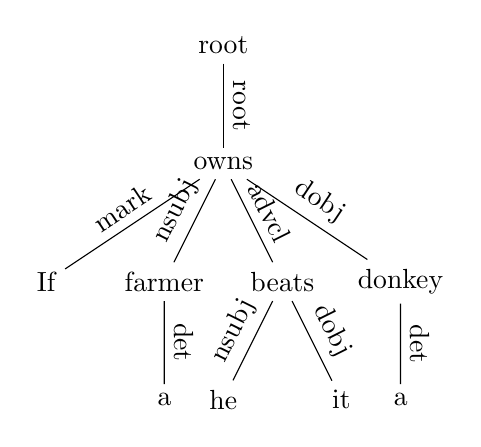
\begin{tikzpicture}[grow=down, sloped]
\node {root}
    child {
        node {owns}
        child {
            node {If}
            edge from parent
            node[above] {mark}
        }
        child {
            node {farmer}
            child {
                node {a}
                edge from parent
                node[above] {det}
            }
            edge from parent
            node[above] {nsubj}
        }
        child {
            node {beats}
            child {
                node {he}
                edge from parent
                node[above] {nsubj}
            }
            child {
                node {it}
                edge from parent
                node[above] {dobj}
            }
            edge from parent
            node[above] {advcl}
        }
        child {
            node {donkey}
            child {
                node {a}
                edge from parent
                node[above] {det}
            }
            edge from parent
            node[above] {dobj}
        }
        edge from parent
        node[above] {root}
    };
\end{tikzpicture}
\caption{M1} \label{fig:M1}
\end{figure}


\begin{equation}
NP < NN \$ VP
\end{equation}

An NP over an NN and w/ sister VP

\begin{equation}
NP < (NN < dog) \$ (VP <<\# (barks > VBZ))
\end{equation}

An NP both over an NN over `dog' and with
a sister VP headed by `barks' under VBZ

\subsection{Coreferences}
Coreferences (or anaphora) is essential in order to create advanced discourse, since it is what allows us maintain a topic beyond the first mention. Without coreferences we couldn't even express simple logical statements such as transitivity: `a man's brother's brother is his brother' etc.

Identifying coreferences (or resolving anaphora) is hence an important part of converting natural language into logic. The issue is not touched upon in Visser's paper, which casually sidesteps the problem by assigning variables to all mentioned entities.

For the subtask of resolving simple pronouns a solution could be to work in terms of subjects, objects, indirect objects and so on. However if not earlier, this certainly fails for pronouns separated from their antecedent by sentence boundaries. Also we want to resolve other kinds of coreferences, such as `John, the farmer, owns a donkey', where `the farmer' and `John' refers to the same entity.

It quickly becomes clear that the problem is not only syntactical. In the sentence `John and his wife had a farm. He took care of the donkeys' we could substitute `He' with `She' and to change the referent of the pronoun. In this case we need semantic knowledge of genders to proceed.

In my project I have taken advantage of the coreference tagger built into Stanford CoreNLP\cite{lee2013deterministic}\cite{lee2011stanford}\cite{raghunathan2010multi}. In the following section I will summarize the workings of this machine, made to work across large texts as well as simple sentences.

Coreference tagging is one part of computational linguistics where machine learning algorithms still haven't been able to outperform large iterative applications of linguistic heuristics. Of course the procedure assumes (most likely) machine learned postagging and named entity recognition, but the main algorithm is transparent and deterministic.

The idea is to iteratively go over the text with different `sieves'. The below example explains each step with an example I have adopted from \cite{lee2013deterministic}:

\begin{quotation}
John is a farmer. He owned a stubborn donkey.
A girl was looking at the donkey.
``It was my favorite,'' John said to her.
\end{quotation}

\begin{description}
\item[Mention detection]
The first step is to identify all noun phrases (NP) and personal (PRP) and possessive (PRP\$) pronouns. This information is easily pulled from the postree. Notice we also identify nested mentions:

[John]$_1^1$ is [a farmer]$_2^2$. [He]$_3^3$ owned [a stubborn donkey]$_4^4$.\newline
[A girl]$_5^5$ was looking at [the donkey]$_6^6$.\newline
``[It]$_7^7$ was [[my]$_9^9$ favorite]$_8^8$,'' [John]$_{10}^{10}$ said to [her]$_{11}^{11}$.

All mentions are initially assigned to separate entities (entity ids). The entities are also attached information we can easily pull from the postree, such as `a girl: {number: singular, gender: female}' which are used for the following rules.
\item[Speaker Sieve]
The purpose of this first sieve is to link self referring pronouns to speakers. Speakers are identified simply by their connection to verbs such as `say' and proximity to the quotations. In our case the pronoun `my' gets linked to `John':

[John]$_1^1$ is [a farmer]$_2^2$. [He]$_3^3$ owned [a stubborn donkey]$_4^4$.\newline
[A girl]$_5^5$ was looking at [the donkey]$_6^6$.\newline
``[It]$_7^7$ was [\textbf{[my]$_9^1$} favorite]$_8^8$,'' \textbf{[John]$_{10}^{9}$} said to [her]$_{11}^{11}$.

In conversational text we would store information about the speakers in our entities. Thus we could e.g. match mentions of `you' to the speaker of the previous quote we saw.

We also note restrictions for future use, so we don't risk coreferencing an `I' with a `he' etc.
\item[String Match]
The second step is to merge entities referred to by exactly the same string. In our case we have two mentions of `John':

\textbf{[John]$_1^1$} is [a farmer]$_2^2$. [He]$_3^3$ owned [a stubborn donkey]$_4^4$.\newline
[A girl]$_5^5$ was looking at [the donkey]$_6^6$.\newline
``[It]$_7^7$ was [[my]$_9^1$ favorite]$_8^8$,'' \textbf{[John]$_{10}^{1}$} said to [her]$_{11}^{11}$.
\item[Relaxed String Match]
This third sieve doesn't get activated by our example. It will try to remove relative clauses and other text following the head word of a mention, and do an exact match of the result. For example [John] and [John, whose donkey loves him] will correctly be merged.

Like the `String Match' sieve, we are not doing anything fancy here, and we will incorrectly coreference the two mentions of `John' in: `[John, who loves donkeys] and [John, who hates donkeys] were brothers.'
\item[Precise Constructs]
The `Precise Constructs' sieve uses a lot of common patterns that link mentions. In our case two `X is Y' patterns are found:

\textbf{[John]$_1^1$} is \textbf{[a farmer]$_2^1$}. [He]$_3^3$ owned [a stubborn donkey]$_4^4$.\newline
[A girl]$_5^5$ was looking at [the donkey]$_6^6$.\newline
``\textbf{[It]$_7^7$} was \textbf{[}[my]$_9^1$ \textbf{favorite]$_8^7$},'' [John]$_{10}^1$ said to [her]$_{11}^{11}$.

Other patterns include acronyms and appositives. For example [Canadian Donkey \& Mule Association] and [CDMA] are linked, because the second is tagged as an acronym and it matches the upper case letters of the first one. An appositive is usually a pattern `X, Y, ...' where Y is another description of X.
\item[Strict Head Match A, B, C] are simply rules strip mentions down to their head word and try to find exact matches. This is similar to `Relaxed String Match', but more radical. In our case we correctly get a link between `a stubborn donkey' and `the donkey':

[John]$_1^1$ is [a farmer]$_2^1$. [He]$_3^3$ owned \textbf{[a stubborn donkey]$_4^4$}.\newline
[A girl]$_5^5$ was looking at \textbf{[the donkey]$_6^4$}.\newline
``[It]$_7^7$ was [[my]$_9^1$ favorite]$_8^7$,'' [John]$_{10}^1$ said to [her]$_{11}^{11}$.

Linking mentions based on their head word is dangerous. e.g. `University of Oxford' and `University of Cambridge' both have `University' as their head word, but are (obviously?) different entities. To combat this a lot of strict rules must be observed. These are however gradually weakened in sieve B and C.
\item[Proper Head Noun Match] could be called `Strict Head Match D'. It is the weakest form of the sieve, as it has only the three constraints: two mentions of the same entity cannot have one included in the other, they cannot contain words referring to conflicting geographical locations, and they cannot have different numbers. e.g. [donkeys] and [at least 5 donkeys].
\item[Pronoun Match]
This last sieve is perhaps the most important one. It is done in the end so that we may have as much data in our entities as possible for matching. Using guesses on gender, number and animacy we can make our final merges:

\textbf{[John]$_1^1$} is [a farmer]$_2^1$. \textbf{[He]$_3^1$} owned [a stubborn donkey]$_4^4$.\newline
\textbf{[A girl]$_5^5$} was looking at \textbf{[the donkey]$_6^4$}.\newline
``\textbf{[It]$_7^4$} was [[my]$_9^1$ favorite]$_8^4$,'' [John]$_{10}^1$ said to \textbf{[her]$_{11}^{5}$}.

As always there are a few constraints put on what can be merged. One rule is that the distance between pronoun and antecedent must be maximum 3 sentences.
\end{description}

After the final step different post processing options are usually performed. For example singleton mentions are often discarded. That would mean we got rid of `a musician' and `my favorite'.

The reason the rules are applied in the order above is to give the most certain rules the highest priority.

The Stanford procedure above is currently the strongest competitor in various coreference competitions.

\subsection{Semantics via dependencies}
This subsection's content...

\section{Implementation (8)}

Incremental dynamics\quote{van2001incremental}

DPL Semantics - Functional Version
DPL Semantics - Relational Version
A state is an element of $D^V$ (function from variables to domain)
In functional semantics a state is a function $D^V -> P(D^V)$
In relational semantics it is a relation $P(D^V x D^V)$

There is not a big first order logic component in my project, but in the following it will often be useful to refer to the following structure

\begin{haskell}
data Prop =
    T | F
  | Not   Prop
  | And   Prop Prop
  | Or    Prop Prop
  | Predi Ref [Ref]
  | Exist Ref Prop
  | All Ref Prop
  | Impl Prop Prop
\end{haskell}

And since we are going to deal with some large computer generated formulas, I've implemented a simple simplification function, which simply applies basic identities for $\top$ and $\bot$, and a combination of De Morgan's laws and the implication identity to eliminate negations.

One interesting part is that since the simplifier has no look ahead, it will sometimes not find all applicable simplifications in one pass. For example
%
\begin{haskell}
simplify (Not (Impl p F)) = Not (simplify (Impl p F))
                          = Not (Not simplify p)
                          = Not (Not q)
\end{haskell}
%
Hence we need to run it a couple of times to get a good result. We can run it until the output doesn't change, or even simpler, just use a function like
%
\begin{haskell}
fexp :: (a -> a) -> Int -> (a -> a)
fexp f e = (iterate (f.) id) !! e
\end{haskell}

\subsection{My implementation of DPL semantics}

Syntactically we will be using the following structure

\begin{lstlisting}
data DPL =
    DT | DF
  | DComp DPL DPL
  | DOr DPL DPL
  | DNot DPL
  | DImpl DPL DPL
  | DExists Ref
  | DPredi Ref [Ref]
\end{lstlisting}

Below are some direct implementation of the semantics for DPL. We use the types
\begin{lstlisting}
type Assignment = [(Ref, Val)]
type Relation = Assignment -> [Assignment]
\end{lstlisting}
This differs from the indirect set of types are used in the earlier formalisms:
\begin{lstlisting}
type Assignment = [(Ref, Val)]
type Relation = Assignment -> Assignment -> Bool
\end{lstlisting}

intuitive

uses well known isomorphism

more direct

The later is very difficult to implement, since the semantics require quantification over all assignments. Like for composition.

\begin{lstlisting}
:: Relation
true = id
false = const []

predi1 :: [Val] -> Ref -> Rel
predi1 f k = filter (\as -> elem (get k as) f)

predi2 :: [(Val,Val)] -> Ref -> Ref -> Rel
predi2 f k l = filter (\as -> elem (get k as, get l as) f)

:: Relation -> Relation
neg r = filter (\as -> null (r [as]))

:: Relation -> Relation -> Relation
comp = flip (.)
impl s r = rnot (s `comp` (rnot r))
\end{lstlisting}
Then comes the most interesting one. To ``randomly reset'' a variable, we have to make sure that we have all assignments in the cross product of new values for the variable and what was there before.

Bum bum. Maybe we should just use a set, then we could overwrite variable assignments
\begin{lstlisting}
exist :: Ref -> [Val] -> Rel
exist k vs ass = [a : as | a <- news, as <- olds]
	where olds = map (filter ((/=k) . fst)) ass
	      news = [(k,v) | v <- vs]
\end{lstlisting}

\subsection{Handling variables}
One thing I haven't found much \cite{visser1999donkey}
Stanford: \cite{lee2013deterministic}
\cite{lee2011stanford}
\cite{raghunathan2010multi}
Coreferences
Using the parse tree and NPs

Something that's very interesting is when to use free variables and when to use bound variables. We can think of free variables as actors known by the context and bound variables as actors introduced in the sentence. So if we had `The farmer had a friend. His name was Anders', we could write the first part as $\exists y \cdot friends(x,y)$ and the second part as $name(y, `Anders')$. This is important to keep compositionality, but it does of course raise the interesting question of how to make sure that the variable for `Anders' in the first and the second sentence is the same.

In addition to being essential for composition, free variables are also very useful for information extraction type sentences. We can imagine writing a curious researcher writing into a search engine `farmers who like donkeys' which translates into $farmer(x) \cdot likes(x,y) \cdot \triangle \cdot \exists y \cdot donkey(y)$.

So how do we know when to include an $\exists$ and when not to?

The coreference parser does however not find entities that are only mentioned once. Hence to make the later processing simpler, we assign those entity to free variable now as well.

The task is slightly complicated by the fact that NP's can be nested, so `The farmer and the donkey' is a NP consisting of two smaller NP's `The farmer' and `the donkey' separated by `and'.

We resolve this by assigning top down, overwriting `word to ref' assignments with fresh variables as we go deeper down the tree. This way, for our short sentence, we might end up with the assignment $\{`The': `y', `farmer': `y', `and': `x', `the': `z', `donkey': `z'\}$

I parse the parse tree using parsec\cite{leijen2001parsec}

\begin{lstlisting}
toMapping :: [Ref] -> PosTree Word -> ([Ref], Map Int Ref)
toMapping vs (Leaf _ _) = (vs, empty)

toMapping vs tr@(Phrase "NP" subs) = (vs', submaps `union` np)
  where np = mapInterval 0 (tsize tr) v
        (v:vs', submaps) = toMapping vs (Phrase "" subs)

toMapping vs (Phrase _ []) = (vs, empty)
toMapping vs (Phrase _ (sub:subs)) = (vs'', p `union` shifted)
  where (vs', subm) = toMapping vs (Phrase "" subs)
        shifted = mapKeys (+tsize sub) subm
        (vs'', p) = toMapping vs' sub
\end{lstlisting}

where $tsize :: PosTree Word -> Int$ gives the number of words in the tree


\subsubsection{Errors}

What do we do when they fail?
Also something from the disjunction chapter.

What if my states always contain the entire domain as their domain. Just add a $\bot$ to the entity set, then everything will be mapped to that as default.

\subsection{Using machine learning}
The $\bowtie$ and $\triangle$ notation makes logic look close enough to natural language that it starts looking tempting to use machine learning methods such as those used in translation to translate.

My main problem here is that such translation requires large amounts of bilingual data. It was out of scope for my project to try create such.

\subsection{Hand coding}
This is not as bad as it sounds. It is similar to Montague and what the Stanford Parser does for dependencies.

\subsection{Examples}
Until now we've been very focused on the same one or two simple sentences. To provide a better test bench for our approach, it is interesting to follow some sentences through the different levels of our approach.

\begin{enumerate}
\item
Some description?
\begin{description}[style=multiline, leftmargin=10.25em]
  \item[Natural language] If a farmer who owns a donkey, he beats it 
  \item[Dependency Graph] ... eh
  \item[Monadic DPL] $\Bowtie \cdot \triangle \cdot \exists x \cdot farmer(x) \cdot \triangle \cdot owns(x,y) \cdot \triangle \cdot \exists y \cdot donkey(y) \cdot \triangle \cdot \Bowtie \cdot beats(x,y)$
  \item[DPL] $\exists x \cdot farmer(x) \cdot \exists y \cdot donkey(y) \cdot owns(x,y) \rightarrow beats(x,y)$
  \item[FOL] $\forall x ( farmer(x) \rightarrow \forall y ( donkey(y) \wedge owns(x,y) \rightarrow beats(x,y)))$
\end{description}

\item The second item
\item
`John wants to marry a Spanish girl'

This one is hard because it is an example of existential non commitment. I bet we'll fail it.
\end{enumerate}

Extract D Testing 
We have already seen some screen shots of the working program; however, we provide two stringent tests 
for our program to ensure it works as intended, along with a test rig to fully analyze the program. In both test 
programs, I will run through the whole series of options available to the user, and ensure its correctness. 
However, I will also demonstrate its ability to visualize code, and hopefully provide valuable insights whilst 
debugging. 
5.1 Simple Program -BFS and DFS using the Visitor Pattern
This test program begins by creating an underlying tree structure…
This kind of debugging is intuitive, and simple to do within this framework. If you have an intuitive 
understanding of what the underlying model in your program should look like, it is fairly straight forward to 
spot bugs like this in  small code samples. Assuming a larger program is in use, the user must delve a little 
deeper into the part of the graph which they suspect the bug to exist in. This is obviously heavily aided by the 
JDT debugger itself. However, this test still shows the usability of the code in a small program, and shows 
that the code can cope with the different types of back links and cross links that can occur in a memory 
graph.

\section{Perspectives/Conclusions (2)}

In the papers it is always assumed that the postree and things are `trivial' or `already sorted', but how do the pieces really stack up when put together?

What I learned

‘a summary of your achievements; a critical appraisal, describing what worked well and what could be 
improved; a discussion of the lessons you have learnt from the project.’
In the ‘Conclusions’ you summarize your work and then stand back from the project and assess it as 
objectively as you can. This shows the examiners that you are capable of evaluating your own work 
according to the standards of the field. It is acceptable to mention areas that were not very satisfactory
because this shows that you have learnt from the experience of doing the project.
There are often three moves starting with a summary of your work, then giving an evaluation, highlighting
both its achievements and limitations and finally the possible future extensions of the work. The Evaluation 
move may also be carried out as part of the Summary. The Conclusion is the mirror image of the 
Introduction, in that it starts with the narrow concerns of the project and widens out to more general 
statements about further work.

Move 1: Summary 
Summarizes the most important aspects of the project work.  

I have successfully developed a novel local type inference algorithm

Move 2: Evaluation
Indicates what the writer considers to be the most valuable aspects of the project and its limitations. Provides 
an assessment of how far the aims of the project have been achieved.

my algorithm is exponential: whereas Gagnon's algorithm is 
polynomial. But experiments of execution time against method length show a typically linear trend whereas 
Gagnon's show a cubic trend

Move 3: Future Work
Gives possible extensions of the project. These suggestions may follow from the limitations mentioned in the 
Evaluation move. 

The greatest scope for future work is extending the application of my algorithm from local type inference to 
global type inference.

Things learned from courses


Should I make my latex file literate haskell? %bhttp://www.haskell.org/haskellwiki/Literate_programming

\lstinputlisting[language=Haskell]{Main.hs}

\section{Acknowledgments}
I would like to thank Samson for guiding me through

the PCFG parser\cite{klein2003accurate}

Érica for linguistic discussions

\newpage
\section{Appendix}
\subsection{Derivation of DPL preconditions}
\begin{align}
\alpha\models\langle\exists x\rangle\phi
 & \leftrightarrow \exists\beta (\alpha[\exists x]\beta \wedge \beta\models\phi) \nonumber\\
 & \leftrightarrow \exists\beta (\forall\omega (\omega \neq x \rightarrow \alpha_{\omega} = \beta_{\omega}) \wedge \beta\models\phi) \nonumber\\
 & \leftrightarrow \exists\beta (\exists\nu (\forall\omega (\alpha[x:=\nu]_{\omega} = \beta_{\omega})) \wedge \beta\models\phi) \nonumber\\
 & \leftrightarrow \exists\beta (\exists\nu (\alpha[x:=\nu] = \beta) \wedge \beta\models\phi) \nonumber\\
 & \leftrightarrow \exists\nu (\exists\beta (\alpha[x:=\nu] = \beta \wedge \beta\models\phi)) \nonumber\\
 & \leftrightarrow \exists\nu (\alpha[x:=\nu]\models\phi) \nonumber\\
 & \leftrightarrow \alpha\models\exists x (\phi) \\
%
\intertext{Here we take $\alpha[x:=\nu]$ to mean the $\alpha$ with $\alpha_x$ assigned to the value of $\nu$.}
%
\alpha\models\langle\psi_1\cdot\psi_2\rangle\phi
 & \leftrightarrow \exists\beta (\alpha[\psi_1\cdot\psi_2]\beta \wedge \beta\models\phi) \nonumber\\
 & \leftrightarrow \exists\beta(\exists\gamma (\alpha[\psi_1]\gamma \wedge \gamma[\psi_2]\beta) \wedge \beta\models\phi) \nonumber\\
 & \leftrightarrow \exists\gamma (\alpha[\psi_1]\gamma \wedge \exists\beta(\gamma[\psi_2]\beta \wedge \beta\models\phi)) \nonumber\\
 & \leftrightarrow \exists\gamma (\alpha[\psi_1]\gamma \wedge \gamma\models\langle\psi_2\rangle\phi) \nonumber\\
 & \leftrightarrow \alpha\models\langle\psi_1\rangle\langle\psi_2\rangle\phi
%
\intertext{c}
%
\alpha\models\langle\psi_1 \cup \psi_2\rangle\phi
 & \leftrightarrow \exists\beta (\alpha[\psi_1 \cup \psi_2]\beta \wedge \beta\models\phi) \nonumber\\
 & \leftrightarrow \exists\beta ((\alpha[\psi_1]\beta \vee \alpha[\psi_2]\beta) \wedge \beta\models\phi) \nonumber\\
 & \leftrightarrow \exists\beta (\alpha[\psi_1]\beta \wedge \beta\models\phi) \vee \exists\beta (\alpha[\psi_2]\beta \wedge \beta\models\phi) \nonumber\\
 & \leftrightarrow (\alpha\models\langle\psi_1\rangle\phi) \vee (\alpha\models\langle\psi_2\rangle\phi) \nonumber\\
 & \leftrightarrow \alpha\models\langle\psi_1\rangle\phi \vee \langle\psi_2\rangle\phi
%
\intertext{d}
%
\alpha\models\langle P(x_1,\dots,x_n)\rangle\phi
 & \leftrightarrow \exists\beta (\alpha[P(x_1,\dots,x_n)]\beta \wedge \beta\models\phi) \nonumber\\
 & \leftrightarrow \exists\beta (\alpha = \beta \wedge P(\alpha_{x_1},\dots,\alpha_{x_n}) \wedge \beta\models\phi) \nonumber\\
 & \leftrightarrow P(\alpha_{x_1},\dots,\alpha_{x_n}) \wedge \alpha\models\phi \nonumber\\
 & \leftrightarrow \alpha\models P(x_1,\dots,x_n) \wedge \phi
%
\intertext{f}
%
\alpha\models\langle\neg\psi\rangle\phi
 & \leftrightarrow \exists\beta (\alpha[\neg\psi]\beta \wedge \beta\models\phi) \nonumber\\
 & \leftrightarrow \exists\beta (\alpha=\beta \wedge \neg\exists\gamma(\alpha[\psi]\gamma) \wedge \beta\models\phi) \nonumber\\
 & \leftrightarrow \neg\exists\gamma(\alpha[\psi]\gamma) \wedge \alpha\models\phi \nonumber\\
 & \leftrightarrow \neg\exists\gamma(\alpha[\psi]\gamma \wedge \gamma\models\top) \wedge \alpha\models\phi \nonumber\\
 & \leftrightarrow \alpha\not\models\langle\psi\rangle\top \wedge \alpha\models\phi \nonumber\\
 & \leftrightarrow \alpha\models \neg\langle\psi\rangle\top \wedge \phi
%
\intertext{e}\nonumber
\end{align}

\bibliographystyle{plain}
\bibliography{refs}

\end{document}
